\documentclass[12pt]{article}
\usepackage{float}
\usepackage{graphicx}
\usepackage{fontspec}
\usepackage{titlesec}
\usepackage{setspace}
\usepackage[style=numeric,backend=biber,sorting=none]{biblatex}
\usepackage[a4paper, total={6in, 8in}, margin=0.5in]{geometry}
\addbibresource{ref.bib}

%%%%%%%% FORMAT
\singlespacing
\setmainfont{Arial}

\titleformat*{\section}{\normalsize\bfseries}
\titleformat*{\subsection}{\normalsize\bfseries}

\pagenumbering{gobble} % Suppress page number

% \titlespacing\section{0pt}{12pt plus 4pt minus 2pt}{0pt plus 2pt minus 2pt}
% \titlespacing\subsection{0pt}{12pt plus 4pt minus 2pt}{0pt plus 2pt minus 2pt}
% \titlespacing\subsubsection{0pt}{12pt plus 4pt minus 2pt}{0pt plus 2pt minus 2pt}


\begin{document}
  
%%%%%%%%% TITLE  
\title{\large Application of micromanipulation techniques in assisted fertilization  \vspace{-2em}}
% \author{\large Yujia Shi\vspace{-1em}}
\date{\vspace{-2.5em}}
\maketitle

%%%%%%%%% BODY TEXT
\section{INTROUDCTION}
micromanipulation is described as a set of tools and techniques that performed on small group of cells or single cells to advacned our understanding in reproductive biology and the development of clinical
methodology.Over the past decade,micromanipulation has played a key role in many scientific discipline, especially in the field of 
assisted fertilization. There is a considerable number of patients unalbe to pregnancy through the conventional in vitro fertilization (IVF) procedure due to failure of fertilization.Various micromanipulation techniques have been developed to assist fertilization, they offer an great effort to address the dilemma of male infertility,they hold great promise for effective diagnosis as well as circumvention of inherited genetic conditions.\medskip


Nowadays, micromanipulation is a field which filled with extensive base of methodology and expertiment, which has been greatly used in variety of reproductive development animal and biology husbandry settings.In the late 1970s, the scientists around the world start to consider the application of micromanipulative techniques in human clincal reproduction. After Steptoe and Edwards have made sucess in  
the  generation an offspring by the conception of in vitro fertillisation, marking a tunning point for assisted reproduction  and  in vitro fertilization in human,since from this event ,various groups all over the world begin to invest more time and efforts in the idea of in vitro fertilization by introducing more complex  techniques of oocyt and embryo manipulation, which bring the hope for patients with severely impaired sperm characteristics, making the sperm more closer or into the ovum.However,to date, there  a relatively large group of patients with poors permatozoal function still can not achieve pregnancy.The remaining failure can be ascribed to the sperm cells are not able to penetrate the zona pellucida and integrate with oolemma. Several procedures have been introduced to  increase the interaction between sperm-egg interaction in the past time such as 

\begin{itemize}
    \item [1)] 
    Either raising the sperm content within the inseminating suspension or decresing the total mass of the insemination medium via the use of microdrops.
    \item [2)] 
    Improving the method of selecting candidate sperm for the purpose of gaining more spermatozoa with normal motibility
    \item [3)]
    facilitating the contact between spermatozoa and moility enhancer as well as isolating the oocyte from the surrounding cumulus cells
\end{itemize}
The above of procedures will be beneficial to treat moderate oligoasthenospermia, but have failed to promote the fertilization in those patients with severely compromised semen parameters.\medskip

Zona pellucida is the main obstacle and natural barrier for normal spermatozoa penetrate into mammalian eggs,this is particularly visible when spermatozoa deficient in density, motility and morphology, the penetration capability to penetrate the zona pellucida will be significantly reduced.
Several techniques have been developed to bypass this thick oocyte's coat.Remove entirely of the zona pellucida exposing spermatozoa to oocyte,however,which may result in low rate of fertilization as well as impair the develpment and survival of the preimplantation embryo.The emergence of micromanipulative techniques designed to enable zona pellucida reaching the oocyte without removal of the entire zona pellucida, which offer some advacne.\medskip


The method Zona drilling was completed through acidic Tyrode’s (AT) medium to create a hole in the zona pellucida, enabling access to oocyte plasma membrane.A similar method to zona drilling is partial zona dissection (PZD) which bring the sperms closer to the female gamete by using mechanical forces to partial open up the human zona pellucida, thereby increasing the interacton between sperm and the oolemma of the oocyte.The partial zone dissection is effective for those oligozoospermic patients,but not meant for asthenozoospermia patients with severse semen problems or immunological infertility.A more direct way to assist the fertilization process is the method called  subzonal insemination (SUZI),which involves in the process of placeing fewer spermatozoas straightly  into the perivitelline space,to avoid the incidence of polyspermy.The appearance of subzonal inseminating is somewhat successful, as which have been applied successfully to treat even male with severely impaired sperm characteristics such as impaired progressive motility.Thus,it is superior to partial zona dissection.\medskip

The dominant progression in the field of assisted fertilization was Intracytoplasmic sperm injection (ICSI).There is doubt that intracytoplasmic sperm injection is currently most outstanding  accomplishment in the field of assisted which is a well established method 
widely used  in assisted reproductive development  and  to be the treatment of choice over zona drilling, paritcal zona dissection and subzonal insemination to treat man with low sperm quality and qunatity as well as non-male factor infertility. \medskip

Intracytoplasmic sperm injection was dervied from the conventional in vitro fertilization (IVF),but there is slightly difference between ICSI and IVF. Intracytoplasmic sperm injection designed to insertion a single spermatozoon no matter its motility or acrosomal status into an oocyte cytoplasm by using a glass micropipette
;while the conventional in vitro fertilization is placing oocytes and sperm in the same Petri dish for the purpose of incubating, and the male gamete will generally fertiliize the oocyte.It is interesting that the Intracytoplasmic sperm injection was established as early as 1966 for non-mammalian gametes expertiment,but have no purpose of assisted fertilization,only demonstrate that the decondensation of sperm nuclear and formation of male pronuclear did not demand for prior interaction between the spermatozoon and the oocyte membranes.
Although ICSI has been applied in the human afterward after multiple experimental testing and improvement in microinjection, this method was still not uilitized extensively,as a consequence of high probaility of damage to oocyte and relative incapability to accomplish the implantation of embryo.It was not until the Free University in Brussels conduct the  subzonal insemination procedure, the sperm unexpectedly penetrated into the oocyte cytoplasm which located at three o'clock position. Due to this accidental success of unexpected sperm injection into the oolemma, giving people a second wind to conduct a serious of clincal investigation to replicate this fortuitous outcome.Finally, the first four pregnancies were generated from the ICSI in 1992, which represented a major breakthrough in the field of assisted fertilization and prove the human oocytees are able to survive the sperm microinjection and afterward give support to the formation of male and female pronuclei.




\section{Indications for ICSI}
Conventional IVF is common techniques to assist fertilization. The biggest achievent that the conventional IVF has made was that the birth of Louise Brown in 1978, but it is as much  less effective when the semen features were extremely beneath the standard values with regard to its concentration,morphology and motility.In other words, it is not the best treatment for severe male infertility.The use of ICSI has been estimated as highly advanced procedure in the treatment  of couples with severe male factor infertility,recently it has been expanded in non-male factor infertility.There still lack of relevant supporting documents and evidence to ascertain the use of 
Intracytoplasmic sperm injection in non-male factor infertility is assocaited with improved fertilization, pregnancy, or live birth rate,thus further substantial analysis is needed.The procedure of ICSI can be summarized as follows A.After the  spermatozoa tail is touced by an injection pipette, the single spermatozoa will unable to mobilize.B
After grasping the immobilized spermatozoa, the injection pipette penetrates the Zona pellucida and oolemma, transferring the spermatozoa inside the oocyte cytoplasm.


\subsection{ICSI for male factor infertility}
Various factors can results in male infertility,inclusive of reduced sperm production,abnormal spermatozoa function as well as  obstruction of the tract of spermatozoa.Among all of these, Azoospermia is defined as the medical condition of complete absence of spermatozoa in the ejaculate due to spermatogenic failure.In humans, aroud about 1\% of the male population affected by the Azoospermia.Azoospermia can be segregate into two broad categories: a genital tract obstruction (obstructive azoospermia)  and  spermatogenic failure (non-obstructive azoospermia).Obstructive azoospermia is a common cause of male infertility which is featured by an blockage or an absence of the reproductive system hamper the spermatozoa entering the seminal plasma before ejaculation.The cause of Obstructive Azoospermia is due to the mutual obstruction of the seminal ducts,In generally, the problem can be solved by retrieveing from the epididymides or testicles, as noraml spermatogenesis in men with obstructive azoospermia is confirmed by histopathological examination. Non obstructive azoospermia is caused by azoospermia absent or seriously decreased sperm generation by the testis,which is highly associated with untreatable testicular disorders.To enable men with obstructive azoospermia and nonobstructive azoospermia have sufficent number of spermatozoa,percutaneous acquisition and open surgery are the two methods commonly used to obtain spermatozoa from epididymal or testicular.The retrieved sperms are then used to fertiliize egg through ICSI techniques.



\begin{figure}[H]
    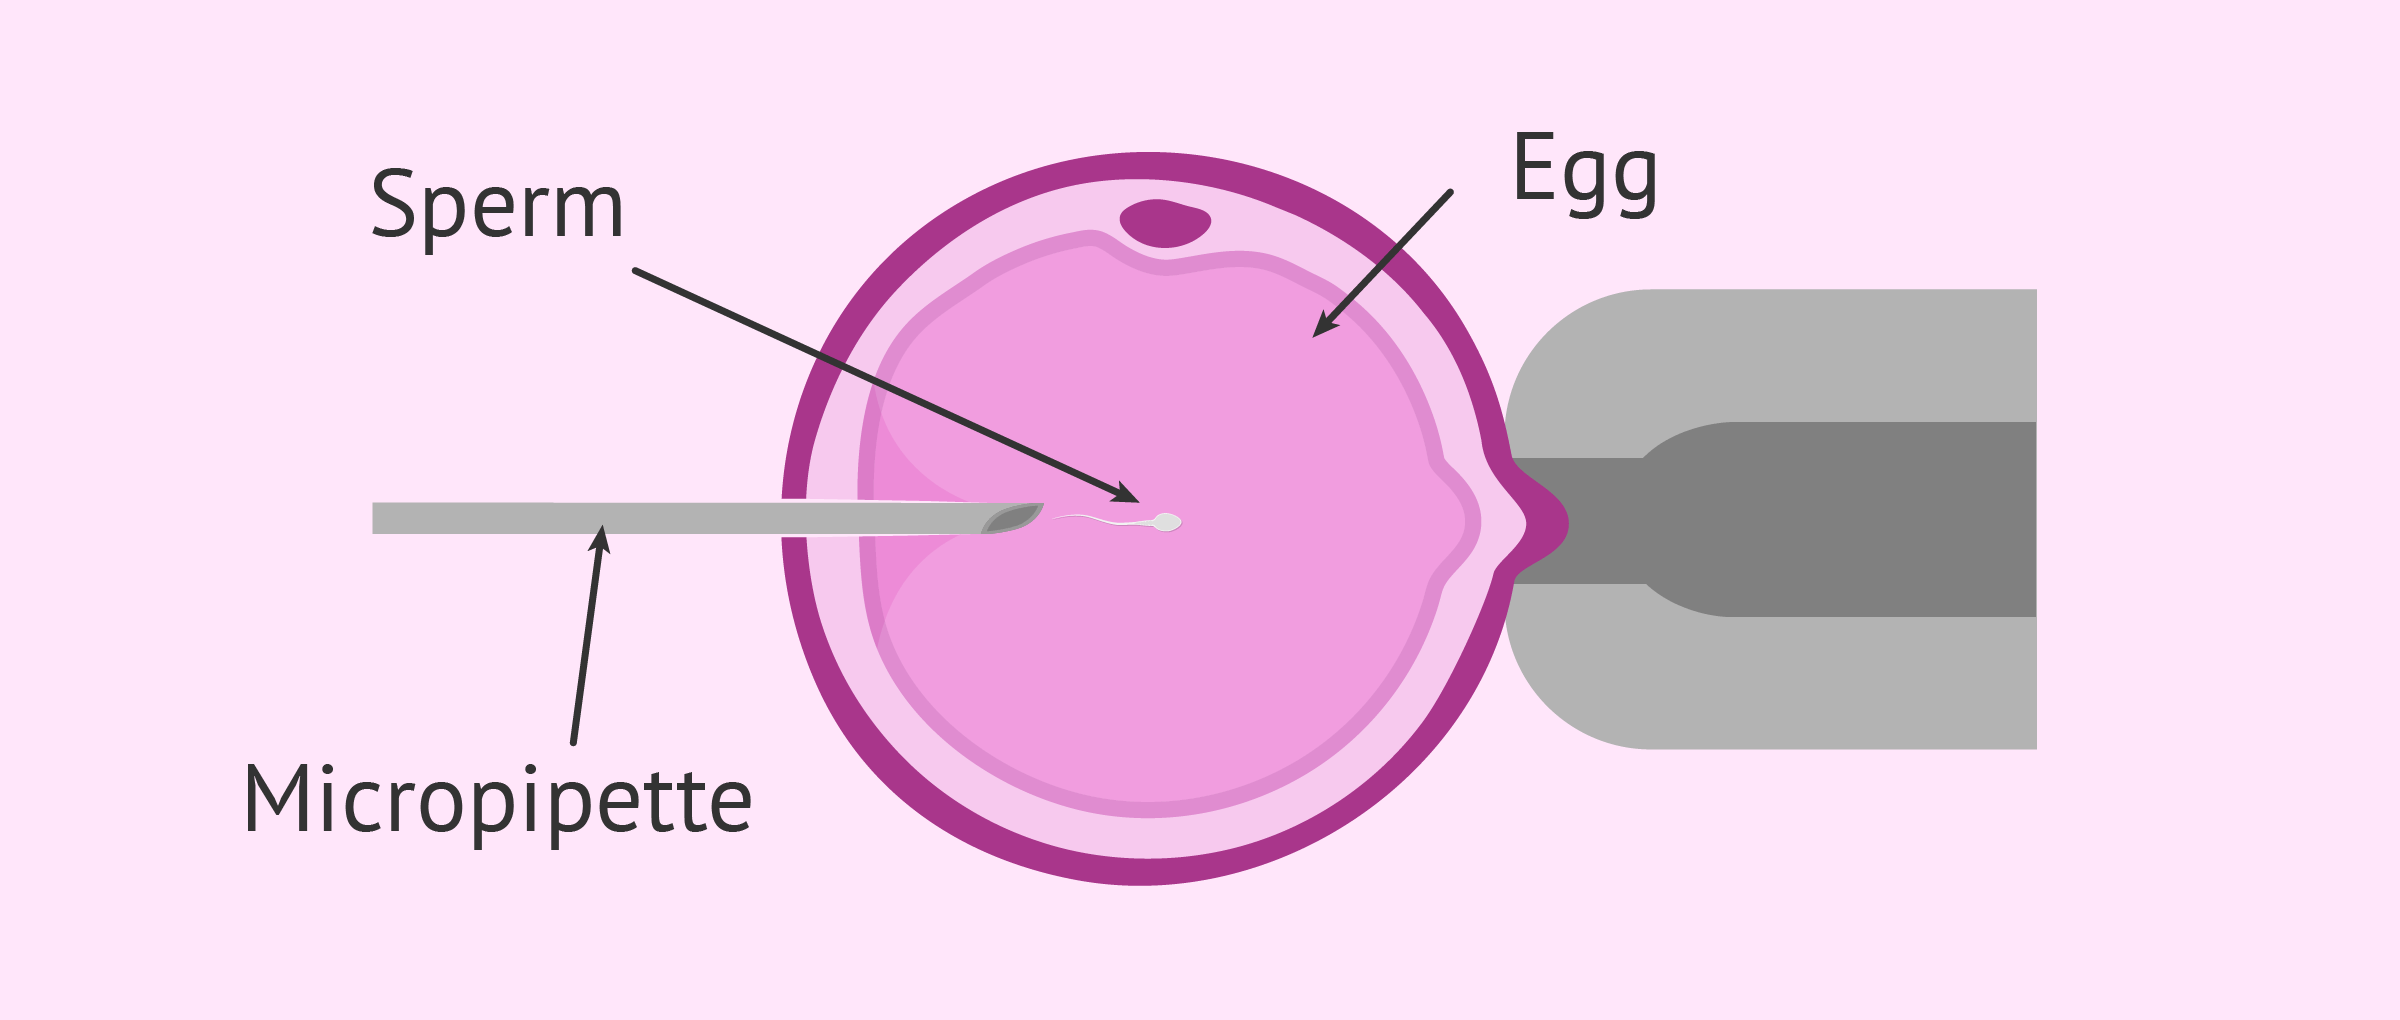
\includegraphics[width=0.9 \linewidth,height=0.5\columnwidth]{/Users/yu-pinglin/Desktop/Essay/6003_kennth.png}
    \centering
    \caption{The 4 pillars for building a sustainable portfolio of
    core facilities.}
\end{figure}

\subsection{LIMITS AND CONCERNS REGARDING ICSI}
As ICSI becomes an standard and most common method of fertilization used for ART.several concerns have been  rasied regarding to its harmful effects on consequent embryo and children.With the aid of ICSI in fertilization,it is possible to bypass the natural selection of the sperm for fertilization, however the sperm with defect characteristics will pass on to the next generation.According to the the resarch report, one fifth of man with azoospermia or severe oligospermia,they have microdeletions in the long arm of the Y chromosome and transmitted to the male offspring, as they are usually the main candidate for ICSI.Apart from the problem of transmitiing genetic defects to offspring, ICSI also casue detrimental effects on the development of embryo, as the process of sperm injection may unavoidably casue physical damages to the oocyte,thereby,influencing the subsequent embryo development.
\section{CONCLUSION}
ICSI has expanded our ability to treat male with severe oligospermia,asthenospermia,and teratospermia without requiring
to requiring sperm undergoes acrosome reaction.In spite of its success, further investigation must address several major
concerns: [1] oocyte damage; [2] the arbitrary selection
of gametes; [3] the genetic integrity of the embryo;
and [4] ensuing healthy live birth.

\emergencystretch=1em
\printbibliography[title=Reference]

\end{document}




